The followed informations introduce the results of two different tests, 
using the KITTI dataset\cite{Geiger}.


In the first test, see Fig. \ref{fig:imgpapercerta}, 
the algorithm makes the tracking of a target, through of a sequence of nine images, with 
a displacement approximately perpendicular to the observer.
\begin{figure}[!hbt]
\centering
  \subfloat[]{\label{fig:imgpapercertaa} 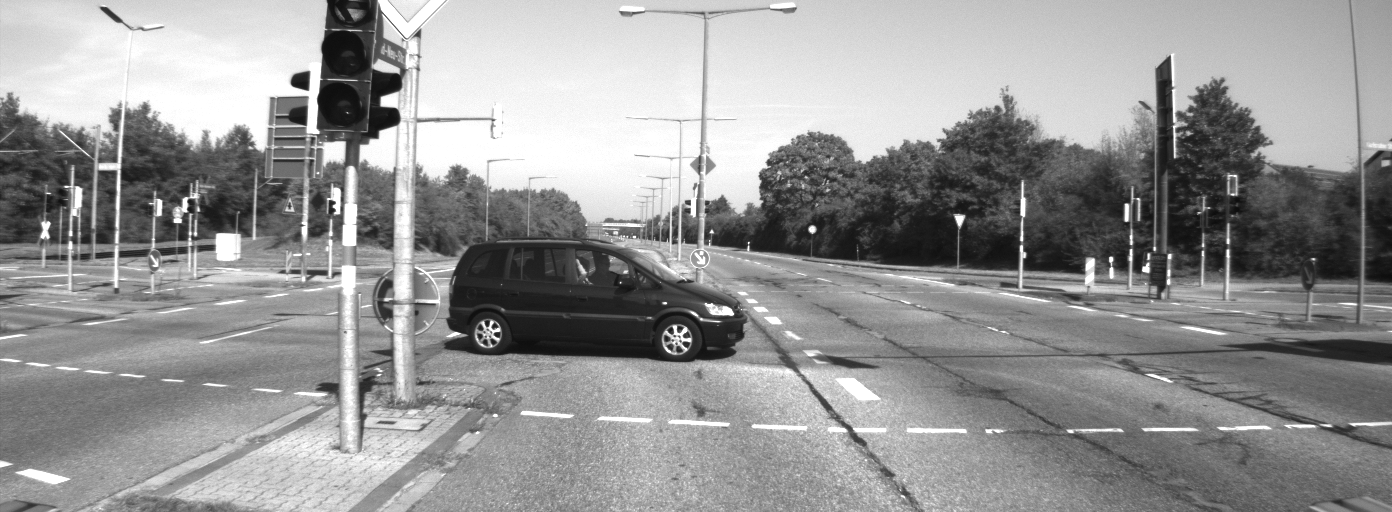
\includegraphics[width=.48\columnwidth]{images/images/0000000000.png}}
  \subfloat[]{\label{fig:imgpapercertab} 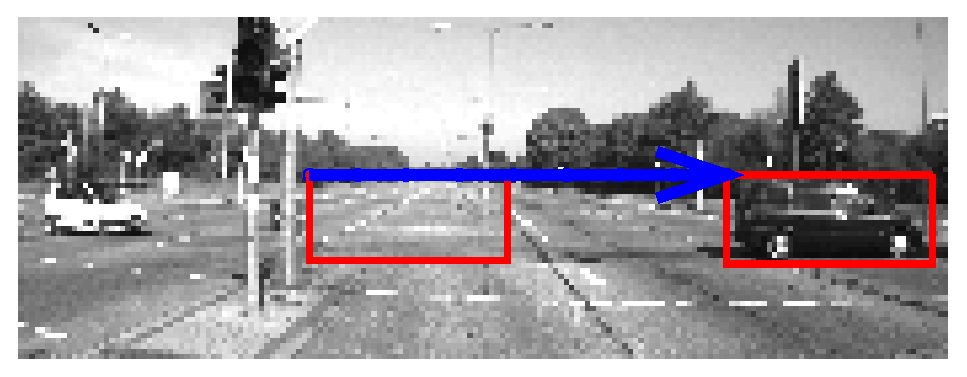
\includegraphics[width=.48\columnwidth]{images/images/img_paper_certa.eps}}
  \caption{The image in (a) represents the target in its initial position 
   and the image (b) shows the vehicle in its final position.}
  \label{fig:imgpapercerta}
\end{figure}
The initial position of target is in the Fig. \ref{fig:imgpapercerta}(a) 
and the final position in the Fig. \ref{fig:imgpapercerta}(b), 
where a vector (in blue) illustrates the resulting trace.
We can observe that there is a small bend in the image 
and it generates a slight change of target perspective. 
This cause the update of the $ROI$, which involves seeing a slight change in area.
The difference among the initial and final values of the departure factor may 
be considered small, as shown in Fig. \ref{fig:res_graph1}.
\begin{figure}[!hbt]
\centering
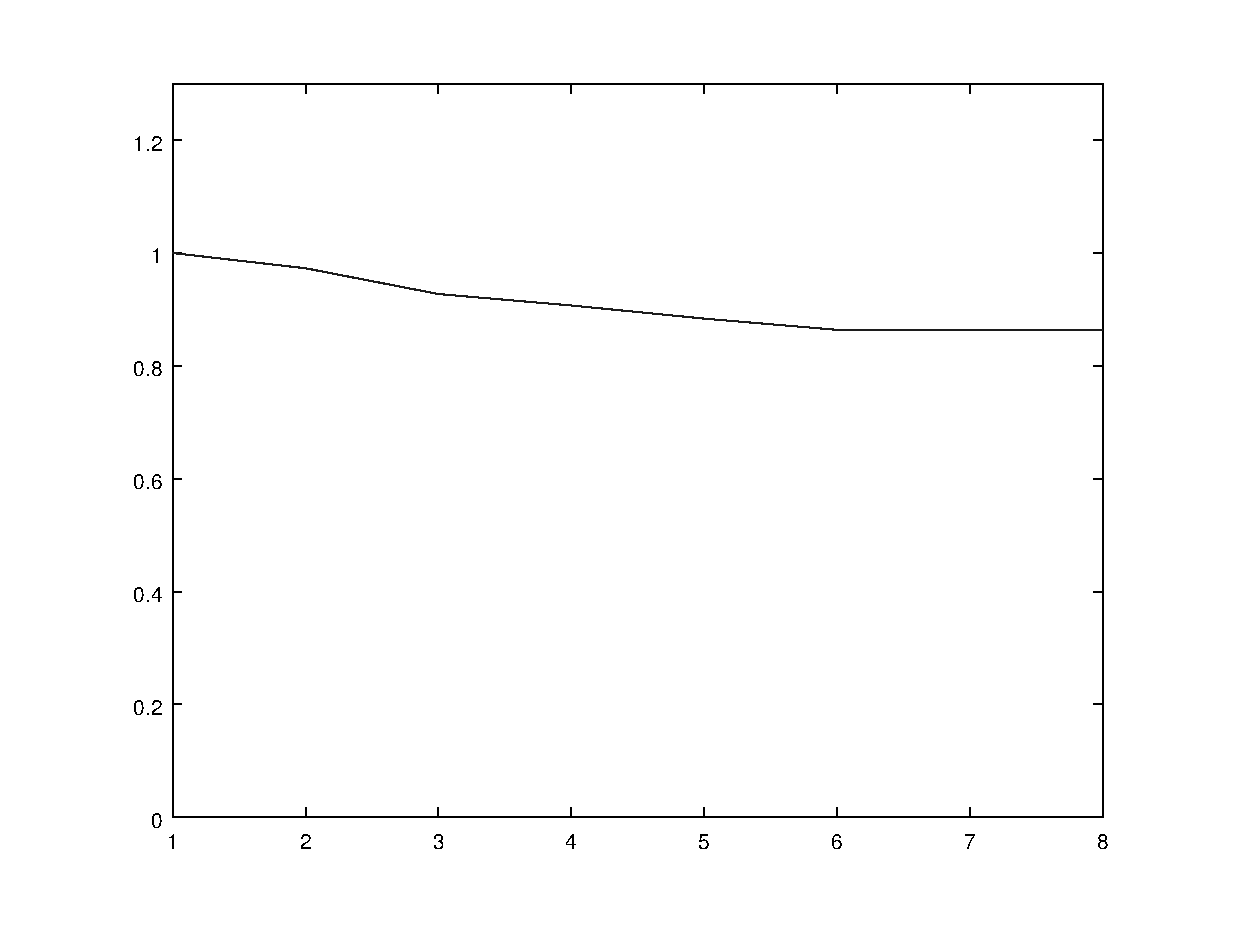
\includegraphics[width=0.8\columnwidth]{images/graph1.eps}
\caption{Departure factor for each image in the test 1.}
\label{fig:res_graph1}
\end{figure}
The Fig. \ref{fig:res_graph1v} shows the velocity of departure factor
to a value $d_0=1$ and a $\Delta t=1$. It is easy to see that the variation
of the departure factor is very small when compared with 1. 
It has a mean departure factor (velocity) of $-0.017020$. This implies in a mean approach of $1.7\%$ of $d_0$
in each one of the nine images.
\begin{figure}[!hbt]
\centering
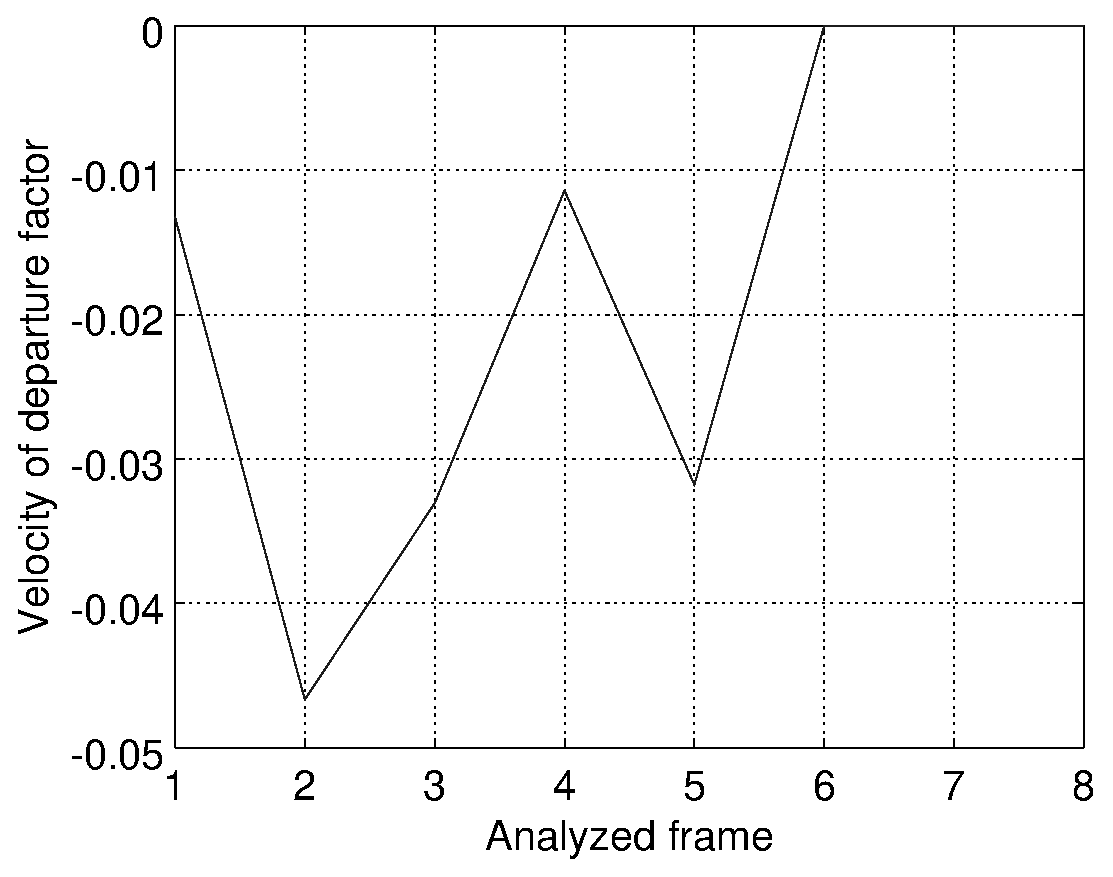
\includegraphics[width=0.8\columnwidth]{images/graph1v.eps}
\caption{Velocity of departure factor for each image in the test 1.}
\label{fig:res_graph1v}
\end{figure}


In the second test, we prove the functionality of algorithm in three dimensions. 
The algorithm compares the images and calculates the departure factor 
based on the target area. The Fig. \ref{fig:target} demonstrates the 
tracking of a target through of $100$ images. The initial and final position of target are 
highlighted with red boxes; and the vector in blue describes the movement of target. 
\begin{figure}[!hbt]
\centering
  \subfloat[]{\label{fig:targeinit} 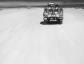
\includegraphics[width=.48\columnwidth]{images/images/351.jpg}}
  \subfloat[]{\label{fig:targeend} 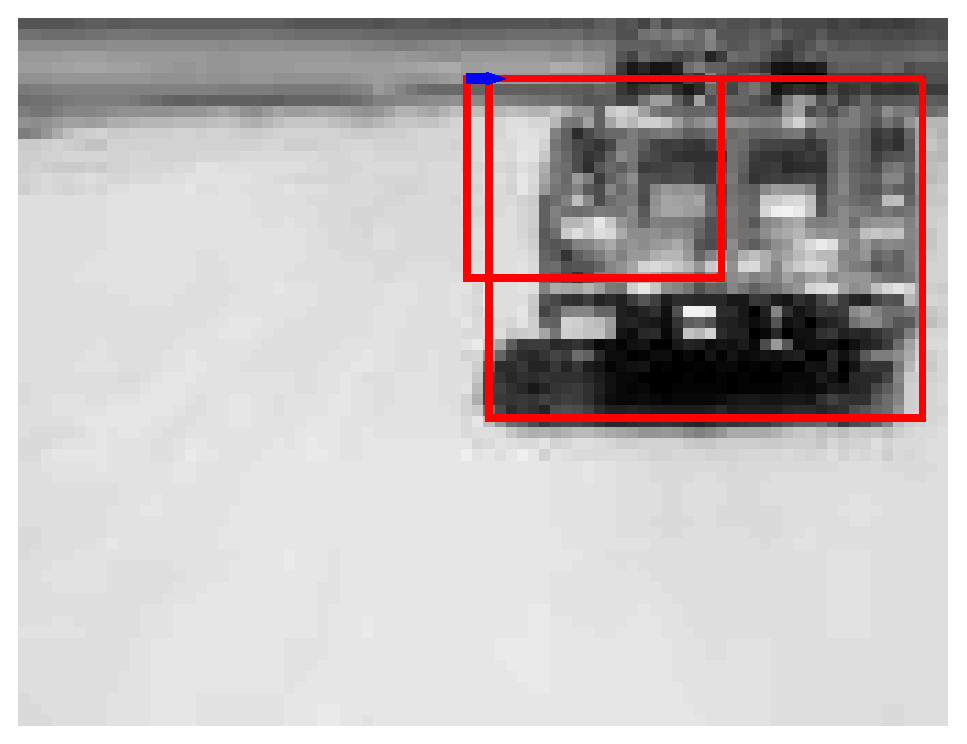
\includegraphics[width=.48\columnwidth]{images/graph2p.eps}}
  \caption{The target in (a) is the initial position and its area is smaller than the target in (b), 
  which represents the final position. The factor is calculate dividing both areas.}
  \label{fig:target}
\end{figure}
In the Fig. \ref{fig:target}, we can observe a significant increase in the target area, and 
its influence to the departure factor.

\begin{figure}[!hbt]
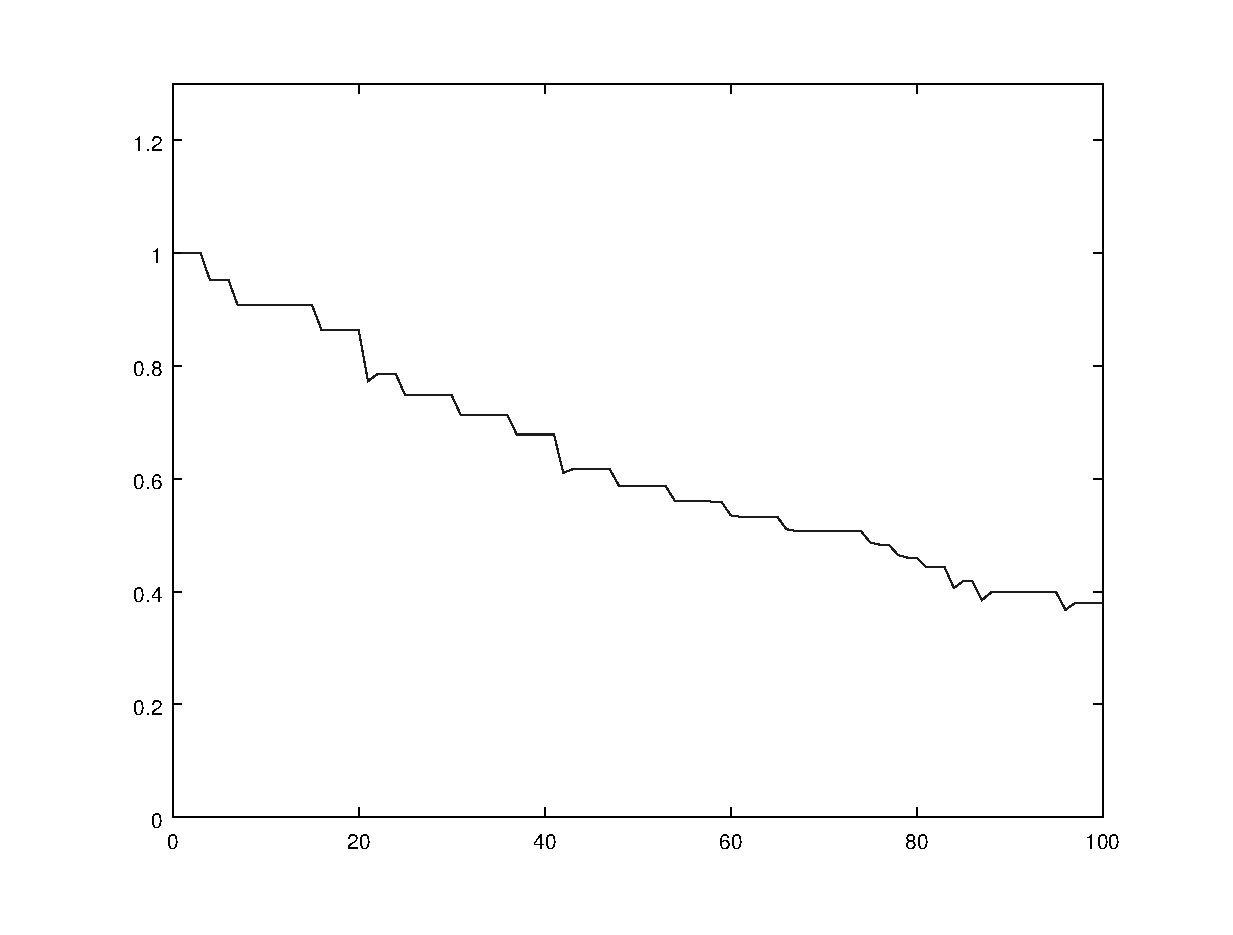
\includegraphics[width=\columnwidth]{images/graph2.eps}
\caption{Departure factor for each image in the test 2.}
\label{fig:res_graph2}
\end{figure}
The Fig. \ref{fig:res_graph2} shows the departure factor in each image
of test 2 and additionally is showed a  fit curve with a piecewise cubic spline 
of 10 breaks. If we interpret the departure factor as the position in each sample time, 
then this describes the relative target position.
So that, in the first image the analyzed target is at a distance $d_0$ 
and in the last image the target is at a distance of $52.42\%$ of $d_0$.
The departure distance decreases in discrete steps because the departure
factor is selected also in discrete steps, then if the target is
between two consecutive analysis layers (scales), the algorithm
approximates the target to the nearest layer. 
\begin{figure}[!hbt]
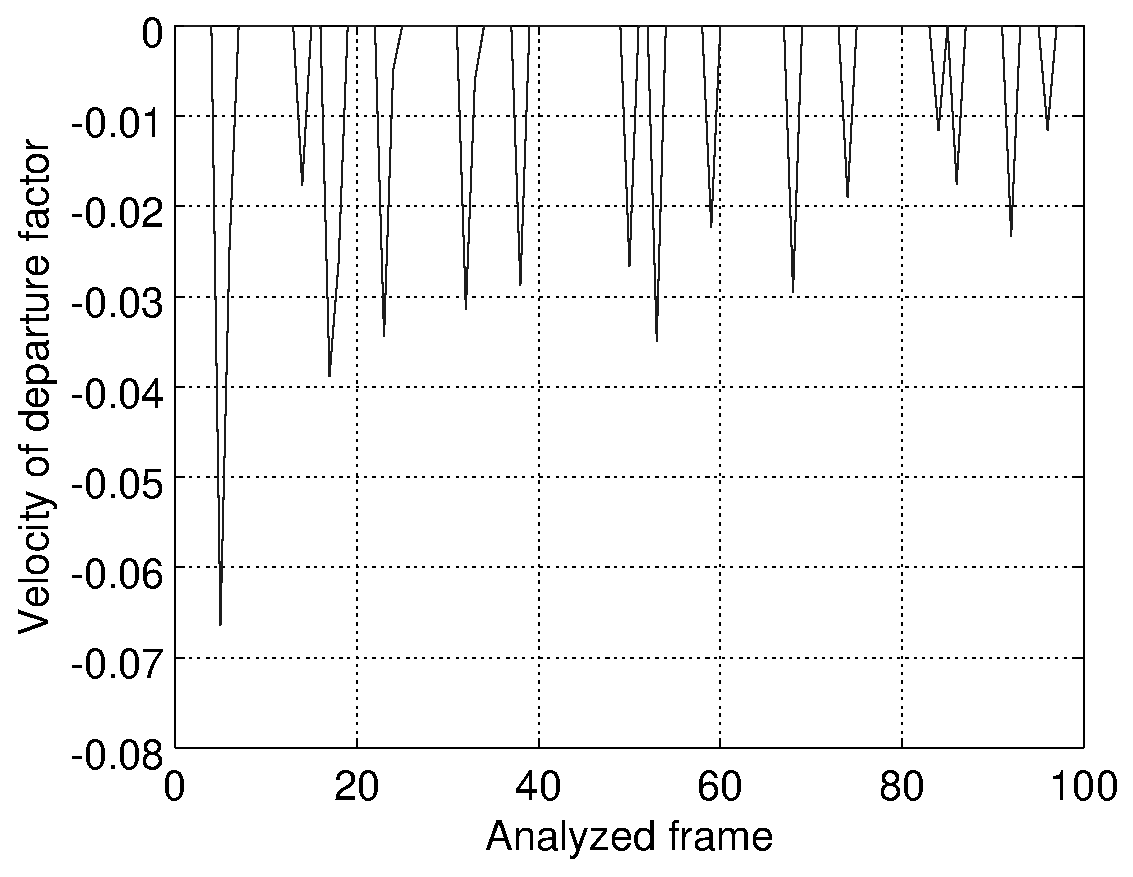
\includegraphics[width=\columnwidth]{images/graph2v.eps}
\caption{Velocity of departure factor for each image in the test 2.}
\label{fig:res_graph2v}
\end{figure}
On the other side, the velocity of departure factor is shown in 
Fig. \ref{fig:res_graph2v}, where the velocity is calculated
to both cases, the departure factor value and the fitted curve, 
being used $d_0=1$ and $\Delta t=1$. The mean value of the departure
velocity is equal to $-0.0048$, and $-0.0050$ to the value from the fitted curve, 
which indicates that the
analyzed  target is in approaching to the observer. Similarly
to the case of the test 1, this mean velocity can be interpret
as a mean approach of $0.48\%$ of $d_0$, by each one of 100 images.
If we compare the test 1 and 2 to the same $\Delta t=1$, it's easy to see
that the departure velocity of the test 2  is lower than the test 1, 
but as the test 2 has more analyzed images (100 images)
the approaching to the observer is greater; 
not to mention that in the test 1, the small number of images 
make  unrepresentative the mean value.




